\section{The Landscape of Rationality for Relations over Finite Words}
\label{sec:preliminaries-automatic-structures-relations}

\subsection{Regularity is Key...}

The class of "regular languages" is remarkably stable, and can either be characterized as the 
languages recognized by either:
\begin{itemize}
	\item deterministic or non-deterministic finite state automata,
	see "eg" \cite[Proposition~1.2.3, p.~7]{Pin2021FiniteAutomata},
	\item two-way finite state automata by Shepherdson-Rabin-Scott theorem
		\cite[Theorem~2, p.~198]{Shepherdson1959ReductionTwoWay}
		\cite[Theorem~15, p.~123]{RabinScott1959FiniteAutomata},
	\item rational expressions by Kleene's theorem,
		see "eg" \cite[Theorem~1.5.11, p.~34]{Pin2021FiniteAutomata},
	\item monadic second-order logic by Trakhtenbrot-Büchi-Elgot theorem,
		see "eg" \cite[Theorem~2.2, p.~32]{Bojanczyk2020MSO}, or
	\item finite monoids,
		see "eg" \cite[\S~1.4.2, p.~19]{Pin2021FiniteAutomata}.
\end{itemize}
Moreover, all transformations between these representations are effective---although some
models can be strictly more succinct.

These equivalences explain why the terms \emph{recognizable language}---meaning implicitly
``recognizable by a finite-state automaton'' or ``recognizable by a finite monoid''---and
\emph{rational language}---meaning ``described by a rational expression''---are used 
interchangeably. In fact, in this thesis as well as in most of the literature,
we will use the generic term "regular language".
However, in more complex settings, for instance subsets of non-free monoids,%
\footnote{Recall that a language is nothing else but a subset of a free
(usually finitely-generated) monoid.}
the equivalence between these classes no longer holds. \cite{Pin2021StackExchange}

The landscape of rationality for $k$-ary relations of finite words ($k \geq 2$) is far more complex than for languages,\footnote{Which can be seen as unary relations of finite words.} as depicted in \Cref{fig:landscape-rationality-relations}. We will briefly present these classes,
although this thesis will only deal with the two most restrictive ones, namely
"recognizable@@rel" and "automatic relations".%
\footnote{It should be noted that the names
of these classes were often coined independently of one another---sometimes defying common sense.
For instance, "automatic relations" are named this way because they correspond to
the relations recognized by some model of automata...
not unlike most of the classes in \Cref{fig:landscape-rationality-relations}.
They are also sometimes named ``regular relations'', which have nothing to do
with "regular functions" and do \emph{not} correspond to the intersection of "regular functions"
with "functional relations", as one would reasonably expect.}
We fix two alphabets $\Gamma$ and $\Sigma$. In the rest of this section, we focus
on relations $\+R \subseteq \Gamma^* \times \Sigma^*$, "aka" transductions.
\begin{figure}
	\centering
	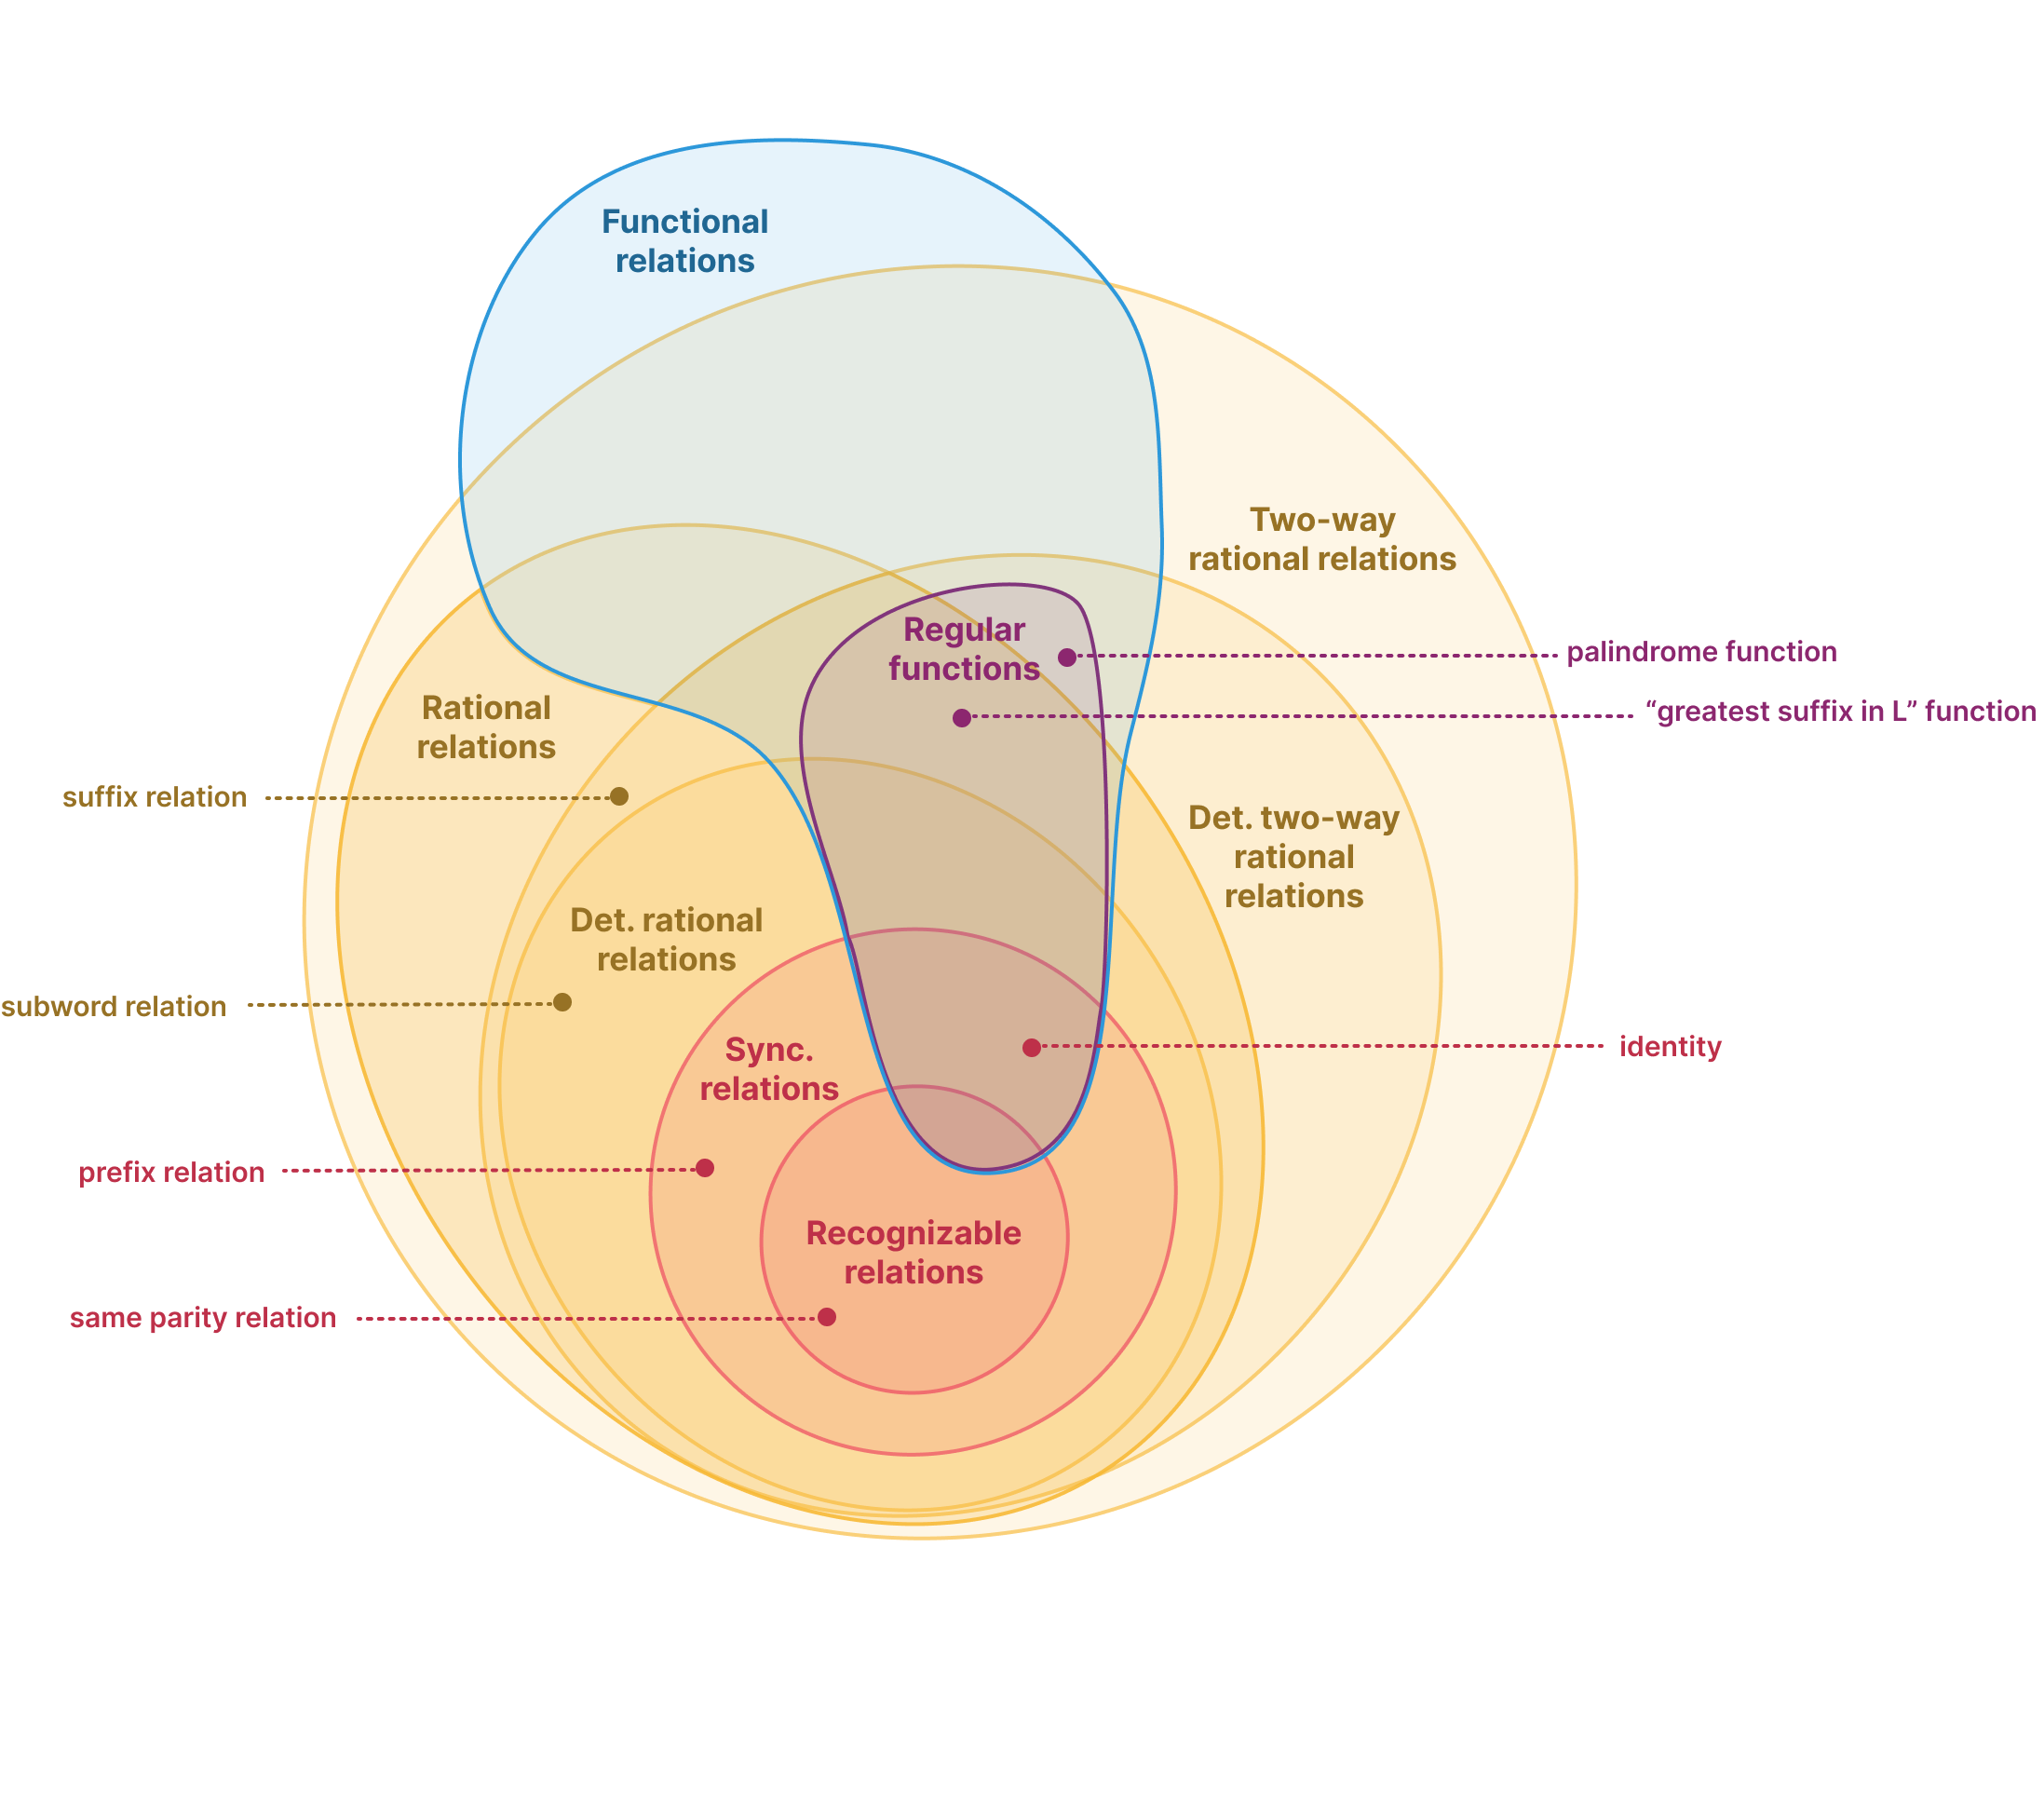
\includegraphics[width=\linewidth]{fig/landscape-rationality-relations.png}
	\caption{
		\AP\label{fig:landscape-rationality-relations}
		The ``landscape of rationality'' for binary relations.
		Dashed regions are empty.
	}
\end{figure}
Often, in the literature, when the terminology ``transduction'' is used,
these relations are thought as functions from $\Gamma^*$ to $\pset{\Sigma^*}$---sometimes
assuming that the input is a singleton, sometimes not---,
and in this case $\Gamma$ (resp. $\Sigma$) plays the role of an ``input alphabet''
(resp. ``output alphabet''). On the other hand, when the terminology ``relation'' is used,
we often take $\Gamma = \Sigma$. This makes little difference since we can often
see a relation $\+R \subseteq \Gamma^* \times \Sigma^*$ as a subset of
$(\Gamma\sqcup \Sigma)^* \times (\Gamma\sqcup \Sigma)^*$
while preserving the notion of ``rationality'' at hand.
Note also that most notions can be trivially extended to $k$-ary relations ($k \geq 3$):
we simply work here with binary relations for the sake of simplicity.


\subsection{Recognizable Relations}

A relation $\+R \subseteq \Gamma^* \times \Sigma^*$ is \AP""recognizable@@rel""
if there exists a "finite monoid" $\?M$ together with a "monoid morphism"
\[
	f\colon \Gamma^* \times \Sigma^* \to \?M,
\]
as well as a subset $\Acc \subseteq M$ "st"
$\+R = f^{-1}[\Acc]$. We denote by \AP$\intro*\REC$ the class of "recognizable relations".%
\footnote{todo: Again, insert some set-theoretic bullshit.}

For instance the \AP""same parity relation""
\[
	\SameParity \defeq 
	\{
		\tup{u,v} \in \Gamma^* \times \Sigma^* \mid
		|u| = |v| \mod{2}
	\}
\]
is "recognizable". Indeed, letting $f\colon  \Gamma^* \times \Sigma^* \to \ZnZ{2}$,
then $\SameParity$ can be written as $f^{-1}[\{\bar 0\}]$.

These relations admit a remarkably simple characterization.\AP
\begin{proposition}[{""Mezei's theorem"", see "eg" \cite[Corollary~II.2.20, p.~254]{Sakarovitch2009Elements}}]
	\!\footnote{\cite[\S~2, ``Notes \& references'']{Sakarovitch2009Elements} mentions
	that this proposition is ``unanimously ascribed to G. Mezei (unpublished)''.}
	\label{prop:Mezei-theorem}
	A relation $\+R$ is "recognizable" "iff" there exists $n\in\N$,
	"regular languages" $\tup{K_i}_{i\in \lBrack 1,n\rBrack}$ over $\Gamma$
	and "regular languages" $\tup{L_i}_{i\in \lBrack 1,n\rBrack}$ over $\Sigma$
	"st"
	\[
		\+R = \bigcup_{i=1}^n K_i \times L_i.
	\]
\end{proposition}

In other words, "recognizable relations" are exactly the finite unions of
"Cartesian products" of "regular languages".
For instance, \[\SameParity =
(\Gamma\Gamma)^* \times (\Sigma\Sigma)^*
\cup \Gamma(\Gamma\Gamma)^* \times \Sigma(\Sigma\Sigma)^*.\]
We provide a slightly more general statement of "Mezei's theorem".

\begin{proposition}
	\label{prop:Mezei-theorem-generalization}
	Let $\B{V}$ be a "pseudovariety of finite monoids"
	and $\+V$ be the corresponding "pseudovariety of regular languages".
	Let $\+R \subseteq \Gamma^* \times \Sigma^*$ be a relation.
	The following are equivalent:
	\begin{enumerate}
		\item there exists a "finite monoid" $\?M \in \B{V}$, a "monoid morphism"
		$f\colon \Gamma^* \times \Sigma^* \to \?M$ and $\Acc \subseteq \?M$
		"st" $\+R = f^{-1}[\Acc]$;
		\item there exists $n \in \N$
		and $K_1,\hdots,K_n \in \+V_{\Gamma}$ and $L_1,\hdots,L_n \in \+V_{\Sigma}$
		"st" $\mathcal{R} = \bigcup_{i=1}^n K_i \times L_i$,
	\end{enumerate}
	in which case we say that $\+R$ is \AP""$\+V$-recognizable@@rel"".
\end{proposition}

When $\B{V}$ is the "pseudovariety@@reglang" of all "regular languages",
we get back \Cref{prop:Mezei-theorem}.

\begin{proof}
	\proofcase{From monoids to products.}
	Assume that $\+R$ is "recognizable@@rel". 
	Then by definition
	\[
		\+R = \bigcup_{z \in \Acc} f^{-1}[z].
	\]
	Observe then that $f(u,v) = f(\tup{u,\varepsilon}\cdot\tup{\varepsilon,v})
	= f(u,\varepsilon)\cdot f(\varepsilon,v)$ for all $u,v \in \Gamma^* \times \Sigma^*$, and hence:
	\[
		\+R = \bigcup_{\substack{x,y \in M\\ \text{"st" } x\cdot y \in \Acc}}
		\underbrace{\{u \in \Gamma^* \mid f(u, \varepsilon) = x\}}_{\defeq \;K_x}
		\times \underbrace{\{v \in \Sigma^* \mid f(\varepsilon, v) = y\}}_{\defeq \;L_y}.
	\]
	Since $M$ is finite, the union is finite, and moreover, each $K_x$ and $L_y$ is
	recognized by $M \in \B{V}$, and hence belong to $\+V$.

	\proofcase{From products to monoids.} If $\mathcal{R} = \bigcup_{i=1}^n K_i \times L_i$ 
		where all languages belong to $\+V$, then let $M_i,N_i \in \B{V}$
		be their "syntactic monoids", $g_i,h_i$ be their
		"syntactic morphism", and $\Acc_i,\Bcc_i$ be their accepting sets.
		Consider the monoid morphism
		\begin{center}
		\begin{tabular}{ccc}
			$\Gamma^* \times \Sigma^*$ & $\to$ & $\prod_{i}(M_i \times N_i)$ \\
			$\tup{u,v}$ & $\mapsto$ & $\tup{g_i(u), h_i(v)}_{i}$.
		\end{tabular}
		\end{center}
		Then $\+R$ is the preimage by this morphism of
		\[
			\bigcup_{i=1}^n \bigl(
			\cdots \times (M_{i-1}\times N_{i-1}) \times
			(\Acc_i \times \Bcc_i) \times (M_{i+1}\times N_{i+1}) \times \cdots \bigr).
		\]
		The conclusion follows from the fact that $\B{V}$ is closed under finite products.
\end{proof}

Both the algebraic definition of "recognizable relations" and
"Mezei's theorem" imply---informally!---that all reasonable problems on
"recognizable relations" are decidable. For instance, from \Cref{prop:Mezei-theorem-generalization},
we get that $\+V$ has decidable "membership" "iff" the class of "$\+V$-recognizable relations"
has decidable "membership".

On the other hand, \Cref{prop:Mezei-theorem} proves that "recognizable relations" are not very expressive.
\begin{corollary}
	\!\footnote{Of course, this property is far from being sufficient
	at characterizing "reflexive relations": note that the proof
	does not even use the "regularity@@lang" of the languages at hand...}%
	\footnote{Of course, another way of proving this result would be
	to apply "Raysey's infinite theorem" to $f\colon \Sigma^* \times \Sigma^* \to \?M$.
	Again, we do not use the fact that $f$ is a "monoid morphism", but simply
	that it is a finite-domain function.}
	\AP\label{coro:infinite-clique-recognizable}
	Let $\+R \subseteq \Sigma^* \times \Sigma^*$ be a "reflexive relation".
	Then $\+R$ contains an infinite clique, "ie"
	there exists an infinite language $L \subseteq \Sigma^*$ "st"
	$\tup{u,v} \in \+R$ for all $u,v \in L$.
\end{corollary}
\begin{proof}
	Indeed, by \Cref{prop:Mezei-theorem}, write $\+R$ as $\bigcup_{i=1}^n K_i \times L_i$.
	Given a word $u \in \Sigma^*$, define $f(u) \in \?2^{2n}$ where
	the $2i$-th (resp. $(2i+1)$-th) bit of $f(u)$ indicates if $u \in K_i$ (resp. $u \in L_i$)
	for all $i$.
	By pigeon-hole principle, there exists a bit-sequence in $\?2^{2n}$ whose preimage
	$L$ by $f$ is infinite. Then pick $u,v \in L$. Since $\+R$ is reflexive, then
	$\tup{u,u} \in \+R$ and so, since $f(u) = f(v)$, we
	have $u \in K_i$ "iff" $v \in K_i$ and
	$u \in L_i$ "iff" $v \in L_i$ for all $i$, and so $\tup{u,v} \in \+R$.
\end{proof}

In particular, this corollary implies that neither the \AP""prefix relation""
${\intro*\prefix} \defeq \{
	\tup{u,v} \in \Sigma^*\times\Sigma^* \mid
	\text{$u$ is a prefix of $v$}
\}$, the \AP""suffix relation""
${\intro*\suffix} \defeq \{
	\tup{u,v} \in \Sigma^*\times\Sigma^* \mid
	\text{$u$ is a prefix of $v$}
\}$, nor the equality relation are "recognizable@@rel".
A similar proof can show that the ""equal-length relation""
$\intro*\equalLength \defeq \{
	\tup{u,v} \in \Gamma^*\times\Sigma^* \mid
	|u| = |v|
\}$.%
\footnote{Note however that \Cref{coro:infinite-clique-recognizable} does not apply since
we assumed there that the input and output alphabets are equal.}


\subsection{Automatic Relations}

"Automatic relations" are a strictly larger class of relations,
and trade some decidability properties to gain in expressiveness.
This is precisely what makes this class interesting to us, and why we will focus
on both "automatic relations" and "automatic structures": while being relatively
expressive, some problems remain decidable.

Given a word $u \in \Gamma^*$ and $v\in \Sigma^*$, we define
its \AP""convolution@@word"" $u \intro*\convol v$ to be the word
$i \mapsto \tup{u_i, v_i}$ of length $\max{(|u|,|v|)}$,
with the convention that $u_i = \pad$ (resp. $v_i = \pad$)
if $u_i$ (resp. $v_i$) is undefined, where $\intro*\pad$ is a new letter called
""blank symbol"" or \reintro{padding symbol}. In other words,
$u \convol v$ is obtained by writing $u$ and $v$ on two left-align horizontal tapes,
adding "padding symbols" at the end of the shorter word if their length differ,
and then reading pairs of letters from left to right.
For this reason, the pair $\tup{a,b}$ is instead written $\pair{a}{b}$.
We let \AP$\Gamma \intro*\convolAlpha \Sigma$ denote the alphabet
\[\Gamma \times \Sigma \cup \Gamma \times \{\pad\} \cup \{\pad\} \times \Sigma,\]
and we let $\intro*\SigmaPair \defeq \Sigma \convolAlpha \Sigma$.

By construction, if $u \in \Gamma^*$ and $v\in \Sigma^*$, then $u\convol v \in (\Gamma\convolAlpha\Sigma)^*$.%
\footnote{When dealing with relations of higher arity, note that $\convol$ is associative up to a trivial
alphabet relabelling.}
For instance
\[
	aba \convol baa = \pair{a}{b}\pair{b}{a}\pair{a}{a}
	\quad\text{ and }\quad
	abab \convol cdd = \pair{a}{c}\pair{b}{d}\pair{a}{d}\pair{b}{\pad}.
\]
We denote by \AP$\intro*\convolRel{\+R}$ the language
$\{ u \convol v \mid \tup{u,v} \in \+R\} \subseteq (\Gamma\convolAlpha\Sigma)^*$.

A (finite-state) \AP""synchronous automaton"" $\+A$ over input alphabet $\Gamma$ and output alphabet $\Sigma$
is a finite-state automaton over $\Gamma\convolAlpha \Sigma$.%
\footnote{In particular, just like for classical automata, we allow for non-determinism
unless otherwise specified.}
We say that $\+A$ accepts the pair of words $\tup{u,v} \in \Gamma^* \times \Sigma^*$ if
it accepts $u \convol v$ as a ``classical automaton''. Similarly, $\+A$ "recognizes@@sync"
$\+R$ if it $\convolRel{\+R}$ is exactly the set of
words of the form $u \convol v$ that are accepted by $\+A$ as a "classical automaton".
A relation is \AP""automatic@@rel"" if it is "recognized@@sync" by a finite-state "synchronous automaton".
We denote by \AP$\intro*\AUT$ the class of "automatic relations".

\begin{remark}
	Note that some words of $(\Gamma\convolAlpha \Sigma)^*$ do \emph{not} correspond to
	encodings of pairs of words, in the sense that they are not of the
	form $u \convol v$ for some $u \in \Gamma^*$ and $v\in \Sigma^*$. 
	This is for instance the case of $\pair{a}{\pad}\pair{\pad}{b}$.
	In fact, $\convolRel{(\Gamma^*\times\Sigma^*)} =
	\{u \convol v \mid \in u \in \Gamma^* \land v\in \Sigma^* \}$ precisely corresponds to
	the words of $(\Gamma\convolAlpha \Sigma)^*$ "st" if some "padding symbol" is seen
	on some tape, then all subsequent symbols on this tape must also be "padding symbols".
	These words are called \AP""well-formed"", and the set of all "well-formed words" over
	$\Gamma$ and $\Sigma$ is denoted by \AP$\intro*\WellFormed[\Gamma,\Sigma]$.%
	\footnote{Of course, when the alphabets are equal, we will write
	$\reintro*\WellFormed[\Sigma]$ instead of $\WellFormed[\Sigma,\Sigma]$.}
\end{remark}

Because of this, some automata that are not \emph{classically} equivalent
become equivalent when seen as "synchronous automaton". For instance, 
both "synchronous automata" of
\Cref{fig:example-synchronous-automaton-prefix-1,fig:example-synchronous-automaton-prefix-2}
"recognize@@sync" the "prefix relation". However, they do not recognize
the same language when seen as classical automaton---for instance, $\pair{\pad}{a}\pair{a}{a}$
is accepted by the automaton of \Cref{fig:example-synchronous-automaton-prefix-1}
but not by the one of \Cref{fig:example-synchronous-automaton-prefix-2}.
Generalizing this example, it is trivial to check that two "synchronous automata"
have the same semantics if, and only if, they have the same
intersection of their semantics, when seen as classical automata, with
an automaton for $\WellFormed[\Gamma,\Sigma]$.

\begin{marginfigure}
	\centering
	\begin{tikzpicture}[shorten >= 1pt, node distance = 1.8cm, on grid, baseline]
		\node[state, initial left, accepting] (q0) {}; 
		\path[->]
			(q0) edge[loop right] node[font=\scriptsize] {$\pair{a}{a}, \pair{\pad}{a}\text{ for }a\in \Sigma$} (q0);
	\end{tikzpicture}
	\caption{
		\AP\label{fig:example-synchronous-automaton-prefix-1}
		A deterministic one-state "synchronous automaton" "recognizing@@sync"
		the "prefix relation".
	}
\end{marginfigure}
\begin{marginfigure}
	\centering
	\begin{tikzpicture}[shorten >= 1pt, node distance = 1.8cm, on grid, baseline]
		\node[state, initial left, accepting] (q0) {}; 
		\node[state, accepting, below=of q0] (q1) {}; 
		\path[->]
			(q0) edge[loop right] node[font=\scriptsize] {$\pair{a}{a}\text{ for }a\in \Sigma$} (q0)
			(q0) edge node[font=\scriptsize, right] {$\pair{\pad}{a}\text{ for }a\in \Sigma$} (q1)
			(q1) edge[loop right] node[font=\scriptsize] {$\pair{\pad}{a}\text{ for }a\in \Sigma$} (q1);
	\end{tikzpicture}
	\caption{
		\AP\label{fig:example-synchronous-automaton-prefix-2}
		A deterministic two-state "synchronous automaton" "recognizing@@sync"
		the "prefix relation".
	}
\end{marginfigure}

Note that, by definition of "synchronous automata", everything that can be done
on classical automata can be done with "synchronous automata",
including determinisation, removal of $\varepsilon$-transitions, completion, etc.
Moreover, observe by the previous paragraph that
the universality of a "synchronous automaton" $\+A$ amounts to 
the universality of the disjoint union of $\+A$ with an automaton for the complement of
$\WellFormed[\Gamma,\Sigma]$.
A similar construction works for the inclusion problem.
\begin{property}
	Inclusion and universality of "synchronous automata" is "PSpace"-complete.
\end{property}
Similarly, the emptiness of a "synchronous automaton" $\+A$ amounts to
the emptiness of the classical automaton obtained by intersecting $\+A$ with $\WellFormed[\Gamma,\Sigma]$.
\begin{property}
	\AP\label{prop:non-emptiness-problem}
	Emptiness and non-emptiness of "synchronous automata" are "NL"-complete.
\end{property}

Similarly to \Cref{fig:example-synchronous-automaton-prefix-1,fig:example-synchronous-automaton-prefix-2},
it is straightforward to prove that the "equal-lenth relation"
and the equality relation are "automatic". As stated before, this class extends
the class of "recognizable relations".

\begin{proposition}
	Every "recognizable relation" is "automatic@@rel".
\end{proposition}

\begin{proof}
	Clearly, "automatic relations" are closed under union: it suffices to do the disjoint union
	of their automata.
	So, to prove this result, it suffices to show that if $K$ and $L$ are "regular languages",
	then $K \times L$ is "automatic@@rel".
	Let $\+A$ (resp. $\+B$) be an automaton recognizing $K$ (resp. $L$). 
	We build a "synchronous automaton" $\+A \otimes \+B$ as follows:
	\begin{itemize}
		\item its states are the pairs of states of $\+A$ and of states of $\+B$,
		\item $\tup{p,q}$ is initial if both $p$ and $q$ are initial,
		\item $\tup{p,q}$ is accepting if both $q$ and $q$ are accepting, and
		\item for every transition $p \transition{a} p' \in \+A$ and $q \transition{b} q' \in \+B$,
			we put a transition
			\[
				\tup{p,q} \transition{\pair{a}{b}} \tup{p',q'},
			\]
		\item moreover, for every transition $p \transition{a} p' \in \+A$, for every $q$,
			we put a transition 
			\[\tup{p,q} \transition{\pair{a}{\pad}} \tup{p',q},\]
		\item and dually, for every transition $q \transition{b} q' \in \+B$, for every $p$,
			we put a transition 
			\[\tup{p,q} \transition{\pair{\pad}{b}} \tup{p,q'}.\]
	\end{itemize}
	By construction, for any $u\in \Gamma^*$ and $v\in \Sigma^*$,
	there is an accepting path in $\+A \otimes \+B$ labelled by $u \convol v$ 
	"iff" $u \in K$ and $v\in L$.
\end{proof}

As often in automata theory, the pumping lemma provides a useful tool to prove
non-regularity, or rather here non-automaticity.
For instance, the "suffix relation" is not "automatic": otherwise,
using the pumping lemma on $a^n \convol b^n a^n$ for some sufficiently big $n\in\N$
would imply that $a^{n+k} \convol b^{n+k} a^n \in \convolRel{\suffix}$ for some $k\in\Np$.

Another useful tool to prove "non-automaticity" is the following one.
Given $I \subseteq \lBrack 1,k\rBrack$,
we say that a $k$-ary "relation" $\+R \subseteq \Sigma_1^* \times \cdots \times \Sigma_k^*$ is
""$I$-locally finite"" if for every $\tup{w_i}_{i\in I} \in \prod_{i\in I} \Sigma_i^*$,
there are only finitely many $\tup{w_j}_{j\not\in I} \in \prod_{j \not\in I} \Sigma_j^*$
"st" $\tup{w_1,\hdots,w_k} \in \+R$.%
\footnote{Note that this is one of the very few statements
that we spell out for $k$-ary relation since its generalization from binary to $k$-ary relations
is not entirely trivial.}
\begin{proposition}[Folklore, see "eg" {\cite[Corollary~8.3,p.~821]{Blumensath2024MSOModelTheory}}]
	Let $\+R \subseteq \Sigma_1^* \times \cdots \times \Sigma_k^*$ be "$I$-locally finite".
	Then there exists a constant $n\in\N$ "st" for every
	$\tup{w_1,\hdots,w_k} \in \+R$,
	\[
		\max_{j \not\in I}{|w_j|} - \max_{i \in I}{|w_i|} \leq n.
	\]
\end{proposition}

todo:example
todo: subword relation

\subsection{Todo}

\begin{itemize}
	\item todo:add polyregular functions.
	\item todo: rename ``synchronous relations'' to ``automatic relations''
	\item todo:the intersection of
	functional relations and two-way rational relations
	collapses to regular functions by
	\cite[Theorem 22, p.~243]{EH2001transduction}.
	\item cite Gaëtan's thesis (chapter 1 for finite words, chapter 8 for infinite words)
	\item mention pebble, marble and whatnot.
\end{itemize}